\documentclass[10pt,twocolumn,letterpaper]{article}

\usepackage[margin=0.74in]{geometry}
\usepackage[T1]{fontenc}
\usepackage[utf8]{inputenc}
\usepackage{lmodern}
\usepackage{amsmath}
\usepackage{amssymb}
\usepackage{booktabs}
\usepackage{graphicx}
\usepackage{xcolor}
\usepackage{enumitem}
\usepackage[hidelinks]{hyperref}

\setlength{\parindent}{1em}
\setlength{\parskip}{0pt}
\setlist[itemize]{leftmargin=1.1em, topsep=2pt, itemsep=1pt}
\setlist[enumerate]{leftmargin=1.2em, topsep=2pt, itemsep=1pt}

\newcommand{\method}{Vision-Panda}
\newcommand{\benchmark}{V-BCOOD}
\newcommand{\sone}{S@1cm}
\newcommand{\stwo}{S@2cm}
\newcommand{\sfive}{S@5cm}

\title{\method{}: Controlled Visual Diversity and Phase-Geometry Diagnostics for Pixel Robot Behavior Cloning}
\author{
Jai Kumar Sharma \and
Manas Ganti \and
Aninditaa Chauhan \and
Shakir Farhan Mohammed
}
\date{}

\begin{document}
\maketitle

\begin{abstract}
Behavior cloning from pixels is simple to supervise but brittle in closed-loop robot control. A practical question is not only whether more visual data helps, but which visual variation should be collected first when demonstrations are limited. We study this question in \method{}, a controlled PyBullet Franka Panda benchmark with 128$\times$128 dual-camera observations, two reaching tasks, four visual diversity axes, and matched in-distribution and out-of-distribution evaluation banks. The benchmark isolates target color, target spatial distribution, external camera viewpoint, and lighting direction/intensity while holding the scripted expert, action interface, and demonstration budget fixed.

Across Scratch CNN, frozen ImageNet ResNet-18, and partially fine-tuned ResNet-18 policies, using 1,056 metric files and 158,400 closed-loop rollouts, we find that visual diversity has a strongly non-uniform value. Color, camera, and lighting shifts are often manageable at loose precision, especially for Scratch CNNs, while spatial distribution shift remains the persistent failure mode. At 50 demonstrations, Scratch CNN achieves 41.1\% \sone{} on color OOD and 57.9\% on camera OOD, but only 2.9\% on spatial OOD. Pretrained encoders do not reliably fix this simulator domain: frozen ResNet features reduce final drift but are much weaker at strict precision, and partial fine-tuning is unstable. Finally, a phase- and geometry-conditioned diagnostic for the hardest obstacle-aware spatial setting raises Scratch CNN OOD \sone{} from 1.3\% to 53.3\%, suggesting that image-only policies fail partly because task stage and obstacle-target geometry are hidden.
\end{abstract}

\section{Introduction}
Visual behavior cloning is an attractive baseline for robot manipulation. It requires only demonstrations, uses a direct supervised objective, and can be implemented with standard image encoders and multilayer perceptrons. Its main weakness is robustness. A policy is trained on expert-visited states, but at test time it acts on states induced by its own previous mistakes. This covariate shift is a classical imitation-learning problem~\cite{ross2011dagger}, and it becomes more severe when the policy must infer task state from raw pixels.

Recent robot-learning progress often attacks this brittleness by scaling data, representations, or policy classes. Large robot datasets expose models to broader variation~\cite{walke2023bridge,khazatsky2024droid,brohan2023rt1}; pretrained visual encoders improve sample efficiency~\cite{nair2023r3m,seo2023mwm}; and temporal or generative policies improve action modeling~\cite{zhao2023act,chi2023diffusion}. These are important directions, but they can obscure a more basic data-composition question: when demonstrations are expensive, which visual variation is worth collecting first?

This question is hard to answer from large heterogeneous datasets because many factors change simultaneously: camera pose, object locations, lighting, backgrounds, objects, robot embodiments, tasks, and teleoperation styles. Broader data can improve generalization without revealing which source of diversity caused the gain. For a practitioner with a fixed collection budget, that causal distinction matters.

We address the question with \method{}, a controlled benchmark for pixel-based behavior cloning under visual distribution shift. The benchmark, which we call \benchmark{} (Visual Behavior Cloning under Controlled Out-of-Distribution Shift), uses a simulated Franka Panda arm in PyBullet~\cite{coumans2021pybullet}. It studies two tasks, direct reaching and obstacle-aware reaching, using two RGB cameras and end-effector position as observations. We vary one visual factor at a time: target color, target spatial distribution, external camera viewpoint, or lighting direction and intensity. For each axis, we compare fixed or narrow training distributions against diverse or wide training distributions, under matched demonstration budgets.

The resulting study makes three points. First, visual OOD difficulty is not uniform. Spatial distribution shift is much harder than color, camera, or lighting shift in this environment. Second, pretrained visual encoders are not a guaranteed answer for simulated pixel control. Frozen ResNet-18 often reduces final drift but has poor strict precision, while partial fine-tuning improves with more data but is inconsistent. Third, the hardest obstacle-aware spatial failures appear to involve hidden task-stage and geometry inference. A diagnostic policy that receives explicit phase and geometry features, while keeping the RGB streams and behavior-cloning loss, sharply improves the hardest spatial OOD case.

\section{Related Work}
\textbf{Imitation learning.}
Behavior cloning is the simplest imitation-learning objective: minimize supervised action prediction error on expert demonstrations. Its limitation is that the learner is trained on the expert state distribution but evaluated on its own rollout distribution. DAgger formalizes this failure mode and motivates closed-loop evaluation rather than relying only on offline loss~\cite{ross2011dagger}. We follow this lesson by evaluating every policy in a 400-step closed-loop simulator rollout.

\textbf{Visual representations for robot control.}
Early visuomotor-learning work showed that representation structure matters for control. Deep spatial autoencoders, graph-structured imitation, and Transporter Networks all introduce inductive biases for spatial manipulation~\cite{finn2016dsae,sieb2020graph,zeng2021transporter}. More recent work uses large-scale pretraining to learn reusable visual features for manipulation~\cite{nair2023r3m,seo2023mwm}. Our experiments test whether an ImageNet-pretrained ResNet-18~\cite{deng2009imagenet,he2016resnet} reduces the need for visual diversity in a controlled simulation domain.

\textbf{Robot datasets and data composition.}
Large datasets such as BridgeData V2, DROID, and RT-1 demonstrate the value of broad robot data~\cite{walke2023bridge,khazatsky2024droid,brohan2023rt1}. Complementary work studies which data factors matter for manipulation generalization~\cite{saxena2025whatmatters,gao2024compositional,xie2023generalizationgap,garcia2023robust}. \method{} is narrower in task scope but more controlled: it changes one visual factor at a time under fixed budgets and closed-loop metrics.

\textbf{Benchmarks and policy classes.}
RLBench and LIBERO provide broad simulator benchmarks for robotic manipulation and transfer~\cite{james2020rlbench,liu2023libero}. ACT and Diffusion Policy show that stronger sequence models can improve manipulation performance~\cite{zhao2023act,chi2023diffusion}. Our aim is different. We deliberately use simple one-step BC policies first so that failures can be attributed to visual data composition and representation, not to a complex policy class.

\section{Benchmark}
\subsection{Tasks and Observations}
The environment is a PyBullet Franka Panda tabletop scene. The robot starts from a fixed arm configuration and acts by predicting a 3D Cartesian delta for the end effector. At every control step the policy observes:
\begin{itemize}
\item a 128$\times$128 external RGB image,
\item a 128$\times$128 wrist/end-effector RGB image,
\item the current 3D end-effector position.
\end{itemize}
The expert is scripted and deterministic given the scene. It produces the target 3D delta action used for supervised training. We study two tasks. In \emph{reach}, the robot moves directly to a cube target. In \emph{obstacle-aware reach}, the robot must route around a static wall-like obstacle before reaching the same target. The second task keeps the observation and action interface unchanged while adding a harder geometric routing problem.

\subsection{Visual Diversity Axes}
The benchmark isolates four axes. The color axis compares a red-only target distribution with a multi-color training distribution and held-out colors at test time. The spatial axis compares a narrow central target distribution with wider workspace support and edge/corner OOD targets. The camera axis compares a fixed external camera with variation in yaw, pitch, and distance, plus more extreme held-out views. The lighting axis compares fixed neutral lighting with varied light direction and intensity, plus extreme held-out lighting. Non-lighting axes use default PyBullet lighting so that explicit lighting changes are not accidentally entangled with color, spatial, or camera experiments.

\begin{table}[t]
\centering
\footnotesize
\resizebox{\columnwidth}{!}{%
\begin{tabular}{lrrr}
\toprule
Split & Datasets & Timesteps & RGB images \\
\midrule
Training bank & 176 & 947,429 & 1,894,858 \\
ID evaluation bank & 48 & 270,446 & 540,892 \\
OOD evaluation bank & 24 & 134,931 & 269,862 \\
\bottomrule
\end{tabular}
}
\caption{Collected dataset scale. Training includes budgets 5/20/50 with seeds 0/1/2 and high-budget 100/200 with seed 0. Each timestep has external and wrist RGB images.}
\label{tab:dataset-scale}
\end{table}

\begin{figure*}[t]
\centering
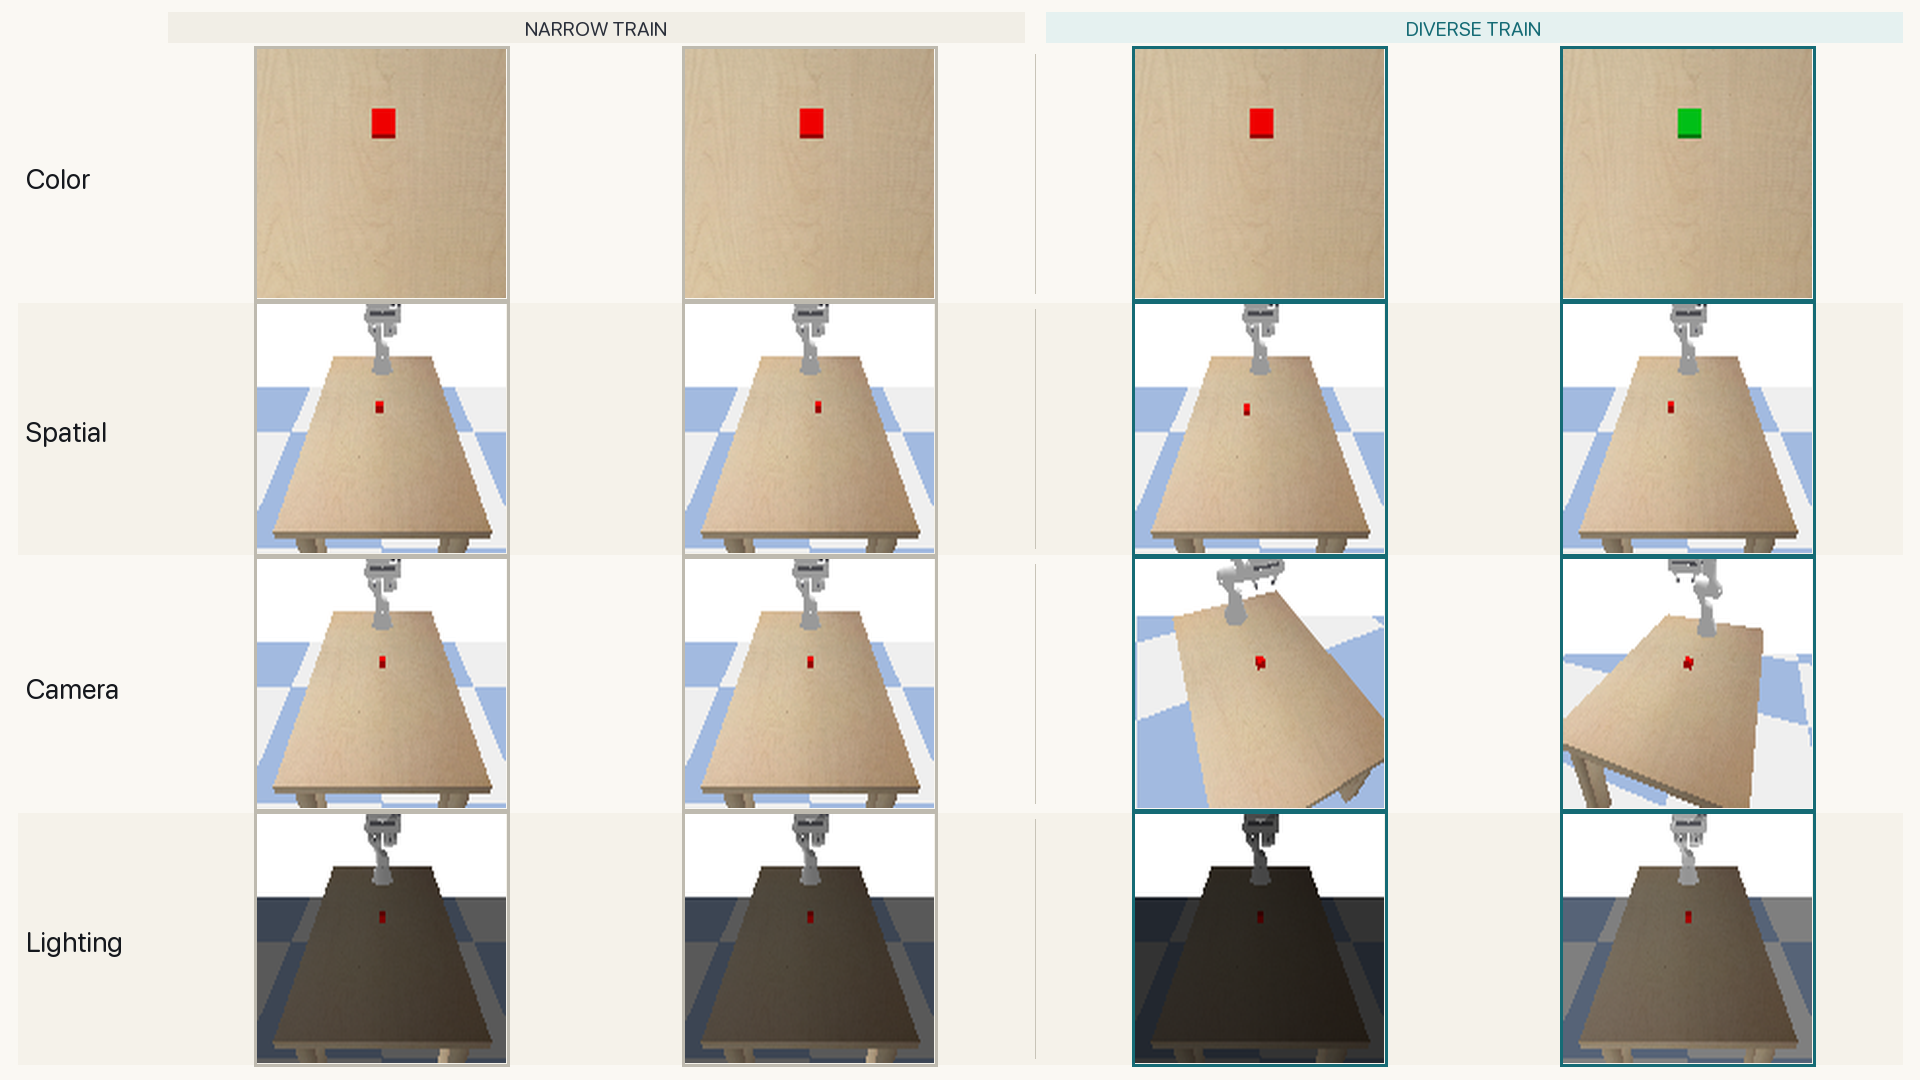
\includegraphics[width=0.94\linewidth]{../results/slide_charts/dataset_diversity.png}
\caption{Public visual overview of the four controlled diversity axes. Fixed or narrow conditions appear alongside broader color, spatial, camera, and lighting variation, while the robot, expert, observation format, and action interface remain fixed.}
\label{fig:dataset-diversity}
\end{figure*}

\subsection{Budgets and Splits}
The primary matrix uses budgets of 5, 20, and 50 expert demonstrations with training seeds 0, 1, and 2. We also run a high-budget extension at 100 and 200 demonstrations with seed 0; these high-budget results are treated as directional. For evaluation, ID scene banks use held-out seeds 200, 201, and 202 from the same distribution, while OOD scene banks use held-out visual conditions with seeds 100, 101, and 102. The collection unit is demonstration count, not transition count, because expert rollouts stop after success.

\section{Policies and Training}
All policies solve the same supervised learning problem. Given two RGB images and end-effector position, the model predicts a 3D delta action and is trained with mean squared error against the scripted expert action. Models are trained for 10 epochs with Adam, batch size 64, and learning rate $10^{-3}$.

\textbf{Scratch CNN.}
The Scratch CNN baseline uses a separate small convolutional encoder for each camera. Each encoder has four convolutional layers followed by adaptive pooling and a 64-dimensional projection. The external embedding, wrist embedding, and end-effector position are concatenated and passed through a two-layer MLP action head.

\textbf{Frozen ResNet-18.}
The frozen encoder policy uses ImageNet-pretrained ResNet-18 features for each camera~\cite{deng2009imagenet,he2016resnet}. The ResNet parameters are frozen, and only projection and policy-head layers are trained. This tests whether generic real-image visual features transfer directly to simulated robot pixels.

\textbf{Partial ResNet-18.}
The partially fine-tuned policy starts from ImageNet ResNet-18 but freezes early layers and trains later residual blocks, projections, and the policy head. This tests whether some adaptation to the simulated domain improves over fully frozen features.

\section{Evaluation}
All reported results come from closed-loop rollouts. At each step, the policy observes fresh rendered images and the current end-effector position, predicts a delta action, and the simulator executes it. The rollout horizon is 400 steps. To avoid loose thresholds artificially ending the episode early, precision evaluation only terminates at 1 mm. We report success using the closest distance reached during the rollout:
\[
S@r = \mathbb{1}\left[\min_t \lVert x^{ee}_t - x^{goal} \rVert_2 \le r \right],
\quad r \in \{1,2,5\}\text{ cm}.
\]
We also report the mean best distance and final distance. Best distance measures whether the policy ever reaches the target neighborhood. Final distance measures whether it stays near the target rather than passing through and drifting away.

\section{Visual-Only Results}
\subsection{Visual Axes Are Not Equally Hard}
Table~\ref{tab:axis50} shows the core multi-seed OOD axis comparison at budget 50. The ranking is clear for Scratch CNN: camera and color shifts are comparatively easy, lighting is intermediate, and spatial distribution is the persistent failure case. Scratch CNN reaches 57.9\% \sone{} on camera OOD and 41.1\% on color OOD, but only 2.9\% on spatial OOD. The same spatial weakness appears for frozen and partially fine-tuned ResNet models.

\begin{table*}[t]
\centering
\small
\begin{tabular}{lrrrrrr}
\toprule
OOD axis at budget 50 & \multicolumn{2}{c}{Scratch CNN} & \multicolumn{2}{c}{Frozen R-18} & \multicolumn{2}{c}{Partial R-18} \\
\cmidrule(lr){2-3}\cmidrule(lr){4-5}\cmidrule(lr){6-7}
 & \sone{} & \sfive{} & \sone{} & \sfive{} & \sone{} & \sfive{} \\
\midrule
Color & 41.1 & 100.0 & 8.3 & 97.7 & 8.6 & 58.9 \\
Camera viewpoint & 57.9 & 91.5 & 9.0 & 85.6 & 4.7 & 56.0 \\
Lighting & 20.6 & 91.2 & 9.2 & 66.2 & 1.9 & 61.0 \\
Spatial distribution & 2.9 & 31.4 & 7.4 & 44.8 & 3.4 & 31.8 \\
\bottomrule
\end{tabular}
\caption{OOD success by visual axis at 50 demonstrations, averaged over both tasks and three seeds. Values are percentages. Spatial distribution is the hardest axis for all three model families.}
\label{tab:axis50}
\end{table*}

\begin{figure*}[t]
\centering
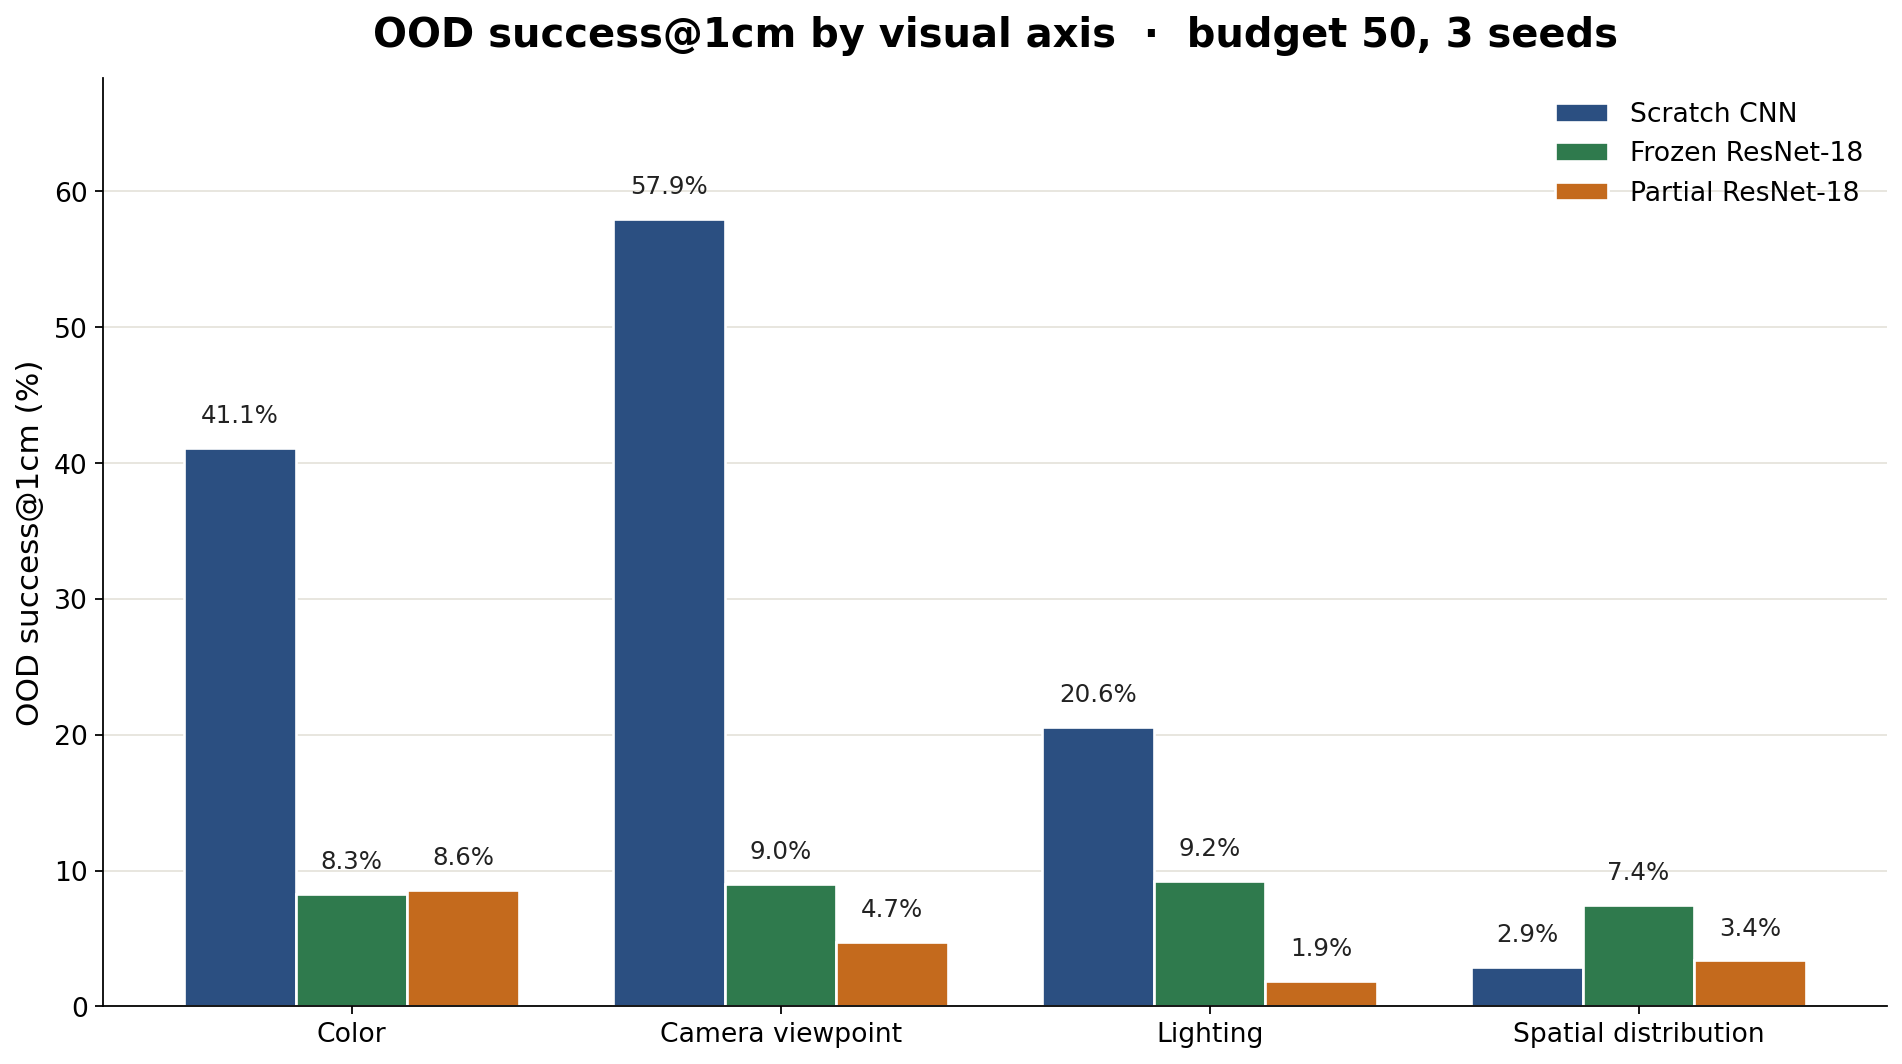
\includegraphics[width=0.95\linewidth]{../results/slide_charts/axis_grouped_bars.png}
\caption{OOD axis ranking across model families and budgets. High-budget 100/200 results use one seed, so they indicate direction rather than final statistical confidence. Spatial OOD remains low even when color, camera, and lighting improve.}
\label{fig:axis-bars}
\end{figure*}

The high-budget extension reinforces the same qualitative trend. At budget 200, Scratch CNN improves to 57.0\% \sone{} on color, 61.7\% on camera, and 50.0\% on lighting. Spatial OOD remains at only 5.2\% \sone{} for Scratch CNN, 15.2\% for frozen ResNet-18, and 6.3\% for partial ResNet-18. More demonstrations help appearance and viewpoint robustness, but they do not remove the spatial bottleneck.

\subsection{Pretrained Encoders Are Not a Clean Fix}
The model-family comparison is more nuanced than ``pretraining helps.'' At 50 demonstrations on OOD rollouts, Scratch CNN obtains 30.6\% \sone{} and 78.5\% \sfive{}, while frozen ResNet-18 obtains only 8.5\% \sone{} but 73.6\% \sfive{}. Frozen ResNet also has lower final distance than Scratch CNN, 23.8 cm versus 40.4 cm, suggesting less severe drift but worse strict precision. Partial ResNet-18 improves with more data, rising from 4.6\% \sone{} at budget 50 to 19.0\% at budget 200, but it remains inconsistent and does not dominate Scratch CNN.

This matters because ImageNet features are not designed for synthetic tabletop control. They may encode useful appearance and shape information, but closed-loop manipulation also needs precise spatial localization and control-relevant geometry. In this benchmark, the small scratch encoder adapts more effectively to the simulator pixels for strict reaching precision.

\subsection{Loose Thresholds Hide Failures}
The gap between \sone{} and \sfive{} is one of the strongest methodological lessons. At budget 50, Scratch CNN reaches 100.0\% \sfive{} on color OOD but only 41.1\% \sone{}. Frozen ResNet reaches 97.7\% \sfive{} on color OOD but only 8.3\% \sone{}. If we reported only a 5 cm threshold, many settings would look solved. The 1 cm threshold and final-distance metric reveal that policies often pass near the target without stabilizing precisely.

Spatial OOD is different. It is low even at loose thresholds: Scratch CNN reaches only 31.4\% \sfive{} at budget 50. This suggests that spatial shift is not just a precision problem; it changes the control geometry enough that policies frequently fail to reach the target neighborhood at all.

\begin{figure*}[t]
\centering
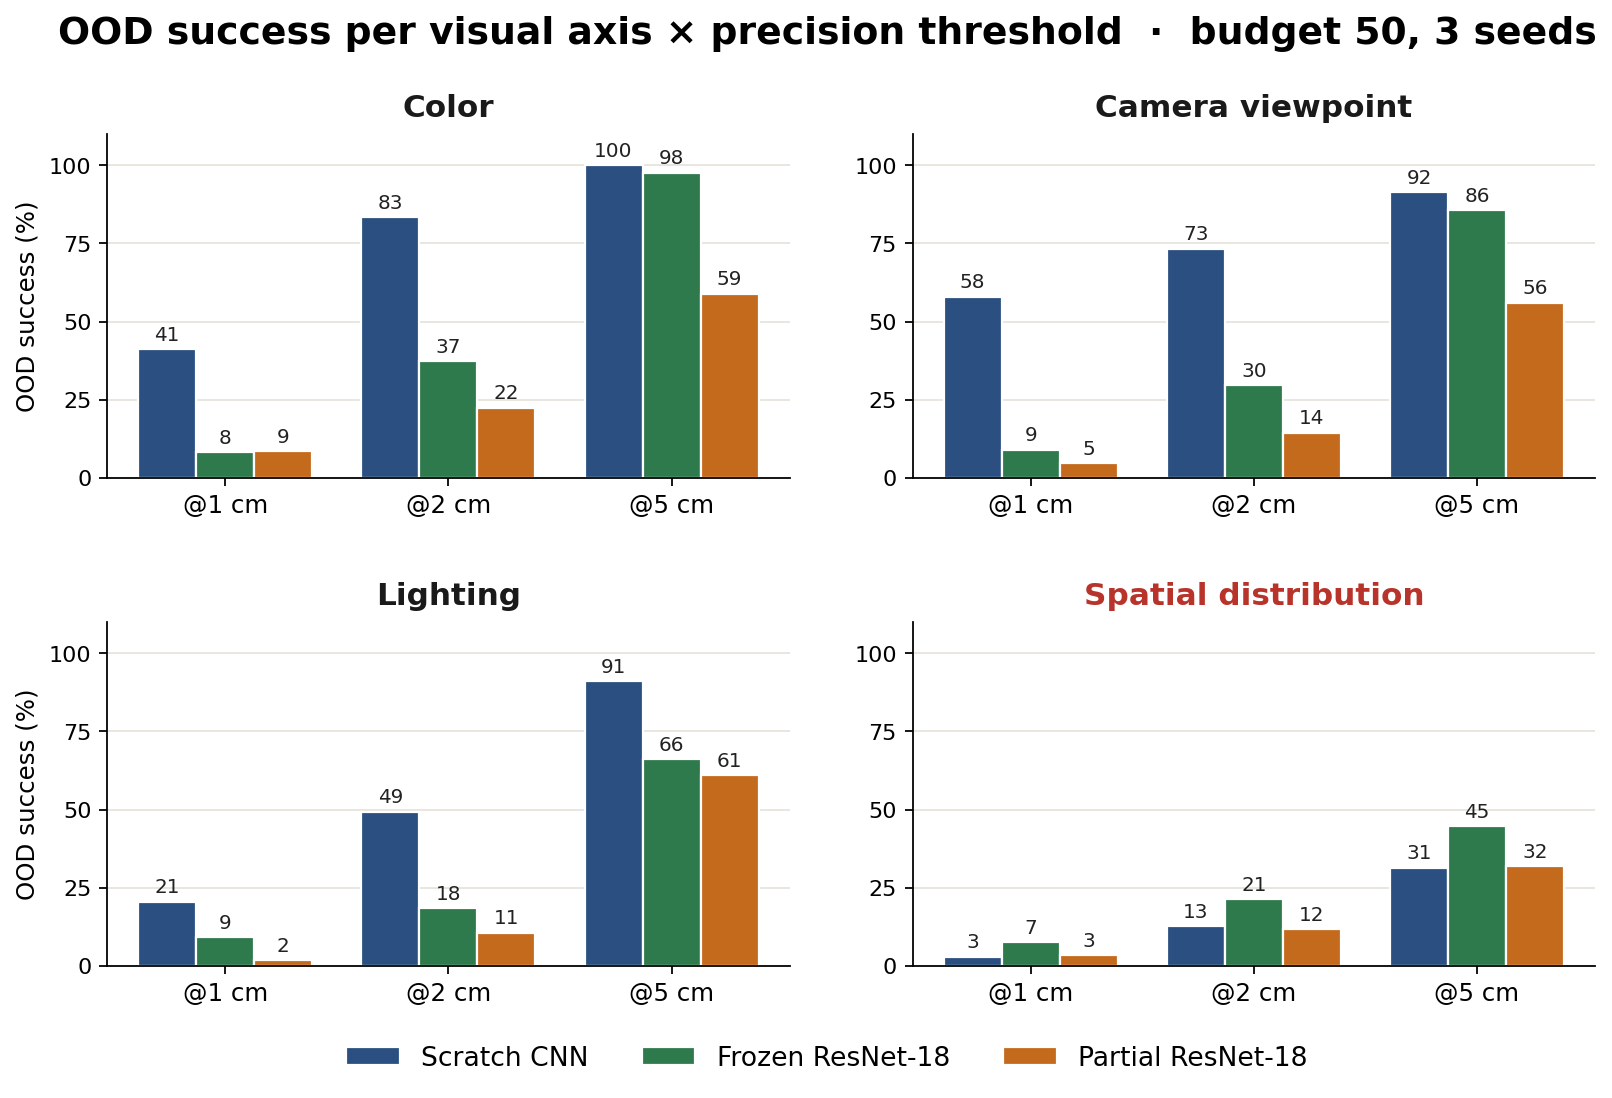
\includegraphics[width=0.86\linewidth]{../results/slide_charts/axis_threshold_grid.png}
\caption{Slide-matched threshold comparison. Several axes look nearly solved at \sfive{}, but strict \sone{} precision is much lower. Spatial OOD remains low even under loose thresholds, indicating a more fundamental geometric control failure.}
\label{fig:threshold-grid}
\end{figure*}

\section{Phase and Geometry Diagnostic}
The obstacle-aware spatial setting is the hardest case in the visual-only matrix. To test whether this is purely a visual diversity problem, we ran a diagnostic intervention. We collected an edge-balanced obstacle-aware spatial dataset and trained policies with the same RGB streams and BC objective, but added an 18-dimensional structured state:
\begin{itemize}
\item one-hot expert phase: \texttt{side\_align}, \texttt{cube\_hover}, or \texttt{final\_descent},
\item target position,
\item obstacle center and half-extents,
\item end-effector-to-target and obstacle-to-target relative vectors.
\end{itemize}
This is privileged information, so we do not present it as a deployable visual-only baseline. Its purpose is diagnostic: if explicit phase and geometry fix the failure, then the image-only policy was missing task-stage and spatial-relation information, not merely more pixels.

\begin{table}[t]
\centering
\footnotesize
\resizebox{\columnwidth}{!}{%
\begin{tabular}{llrrr}
\toprule
Setup & Split & \sone{} & \sfive{} & Final cm \\
\midrule
Visual-only Scratch & ID & 0.0 & 4.7 & 23.08 \\
Visual-only Scratch & OOD & 1.3 & 14.7 & 19.25 \\
Phase+geometry Scratch & ID & 64.7 & 74.7 & 3.27 \\
Phase+geometry Scratch & OOD & 53.3 & 58.7 & 4.23 \\
\bottomrule
\end{tabular}
}
\caption{Diagnostic result on edge-balanced obstacle-aware spatial reaching. Values are percentages except final distance. Adding phase and geometry raises OOD \sone{} from 1.3\% to 53.3\%.}
\label{tab:structured}
\end{table}

Table~\ref{tab:structured} shows the main diagnostic result. Edge-balanced visual-only Scratch CNN does not solve the hard spatial setting: OOD \sone{} is 1.3\%, and final distance is 19.25 cm. With phase and geometry, the same Scratch CNN family reaches 53.3\% OOD \sone{} and reduces final distance to 4.23 cm. This is a much larger improvement than changing the visual encoder family in the same setting.

\begin{figure*}[t]
\centering
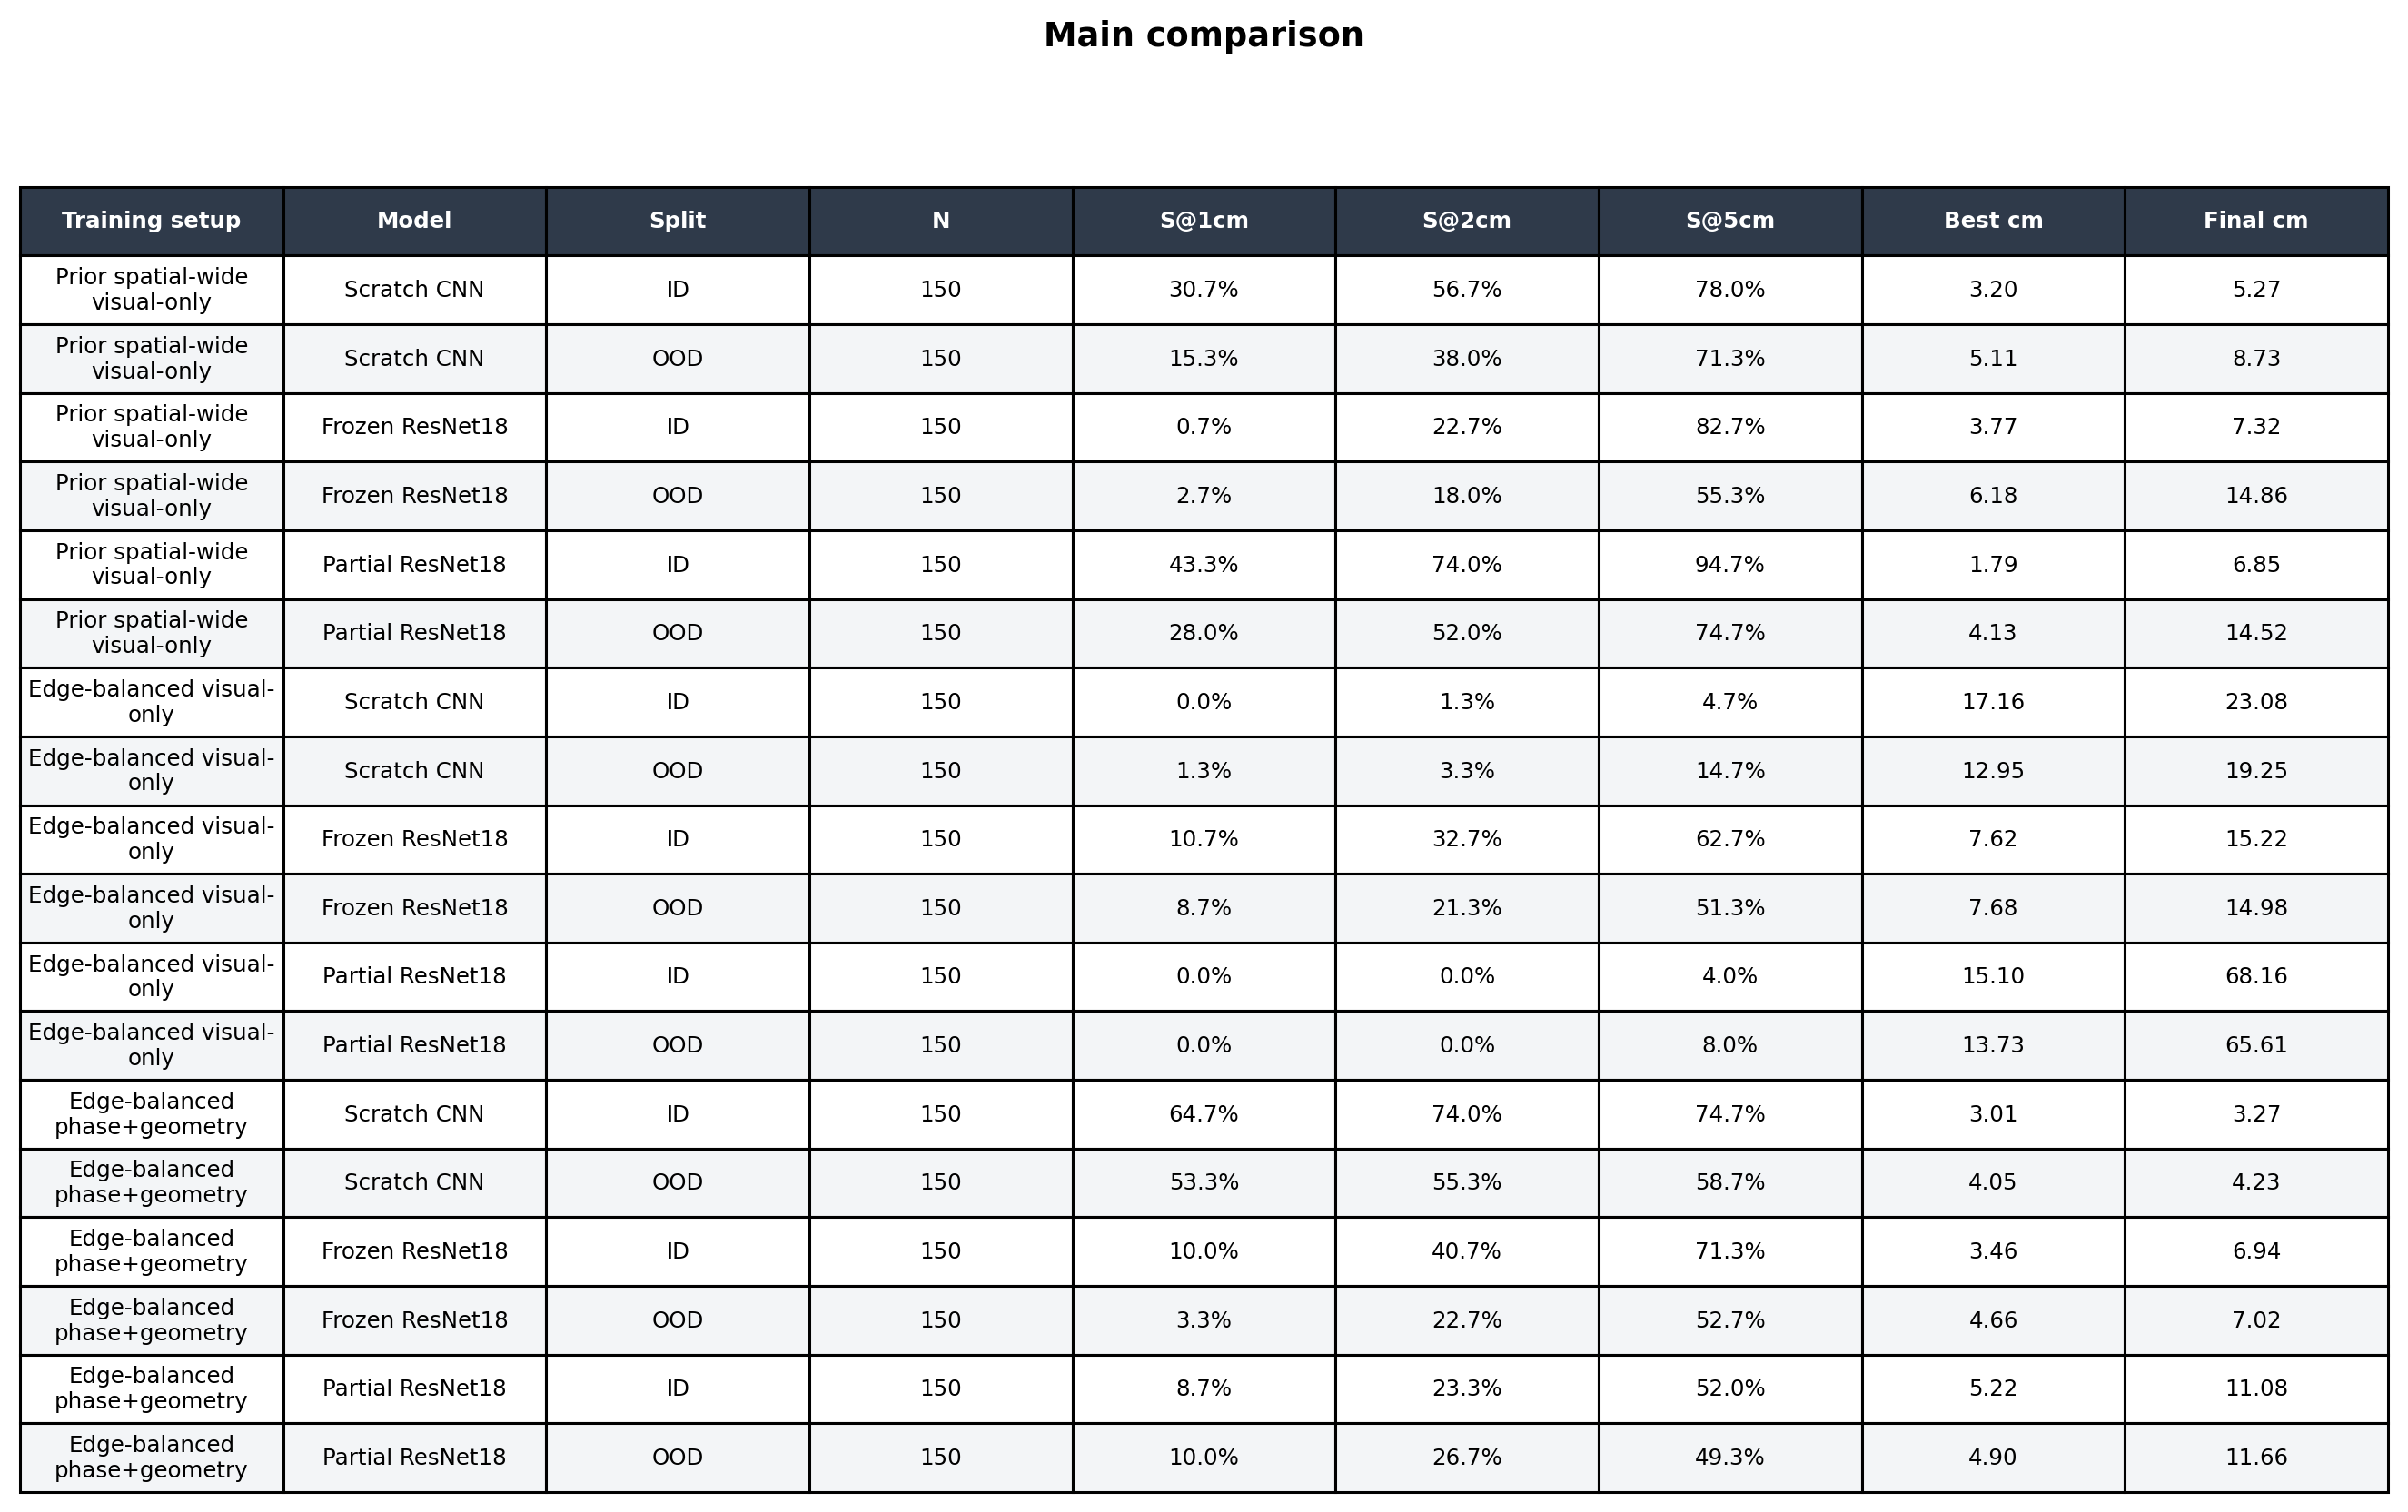
\includegraphics[width=0.95\linewidth]{../results/structured_analysis/main_comparison.png}
\caption{Structured diagnostic comparison for obstacle-aware spatial reaching. Phase+geometry conditioning substantially improves strict precision for Scratch CNN, while frozen and partial ResNet variants remain weaker.}
\label{fig:structured}
\end{figure*}

Ablations clarify what the structured signal contributes. Phase alone fails because it does not locate the target or obstacle. Geometry alone gives excellent loose success and final stability, with 100.0\% OOD \sfive{}, but only 21.3\% OOD \sone{} for full geometry and 6.7\% for target-only geometry. Phase plus geometry gives the best strict precision, 53.3\% OOD \sone{}, but is more bimodal at loose thresholds. This suggests a tradeoff between robust coarse reaching and precise phase-conditioned behavior.

The bucket analysis gives a more concrete interpretation. On OOD corners, visual-only Scratch CNN obtains 0.0\% \sone{} and 0.0\% \sfive{}, while structured Scratch CNN reaches 82.4\% \sone{} and 100.0\% \sfive{}. On edges, it improves from 1.6\% to 62.5\% \sone{}. Interior cases remain harder, improving from 1.4\% to 37.7\% \sone{}. The spatial bottleneck is therefore not uniformly solved, but explicit geometry changes the failure mode substantially.

\section{Discussion}
The main empirical conclusion is that visual diversity is not interchangeable. In this simulator, color, camera, and lighting shifts can often be handled at loose thresholds, while spatial distribution shift remains difficult even with higher budgets and pretrained encoders. This has a practical implication for data collection: if the task requires precise geometric control, broader spatial support and explicit spatial representations should be prioritized over treating all visual augmentation axes as equally valuable.

The representation result is also cautionary. Frozen ImageNet ResNet-18 does not act as a universal visual solution for simulated robot pixels. It is sometimes more stable by final distance, but strict precision is usually worse than Scratch CNN. Partial fine-tuning helps with more data but remains unstable. This does not argue against pretraining generally; rather, it shows that generic image pretraining and closed-loop geometric control solve different parts of the problem.

The diagnostic extension changes the interpretation of the obstacle-aware spatial failure. Additional visual data alone did not solve the hard edge-balanced setting. Explicit phase and geometry did. That result suggests that the policy needs access to control-relevant state structure: where the target is, where the obstacle is, and what stage of the route the expert is executing. In future work, this information should come from deployable perception or structured latent-state models, not privileged simulator state.

\section{Limitations}
The study is intentionally controlled, and that creates limits. First, all experiments are in simulation; we make no direct sim-to-real claim. Second, the task family contains reaching and obstacle-aware reaching, not a broad manipulation suite. Third, demonstration count is fixed but transition count varies because expert rollouts stop after success. Fourth, the high-budget 100/200 results use one seed and should be treated as directional. Fifth, the phase+geometry policy uses privileged information and is best understood as a diagnostic intervention. Finally, conclusions may depend on the specific factor ranges used for color, camera, lighting, and spatial OOD.

\section{Conclusion}
We presented \method{}, a controlled benchmark for studying visual data composition in closed-loop robot behavior cloning. The benchmark isolates four visual diversity axes under fixed tasks, experts, observations, and demo budgets. Across Scratch CNN, frozen ResNet-18, and partially fine-tuned ResNet-18 policies, spatial distribution shift is the clearest and most persistent failure mode. Pretrained encoders do not reliably fix strict precision in this simulated pixel-control setting. A phase- and geometry-conditioned diagnostic sharply improves the hardest obstacle-aware spatial case, indicating that image-only BC fails partly because it must infer hidden task stage and obstacle-target geometry from pixels alone. The broader lesson is that visual diversity helps, but closed-loop robustness also depends on exposing the right spatial and phase structure to the policy.

\begin{thebibliography}{99}
\small

\bibitem{ross2011dagger}
S. Ross, G. Gordon, and J. A. Bagnell.
\newblock A reduction of imitation learning and structured prediction to no-regret online learning.
\newblock In \emph{AISTATS}, 2011.

\bibitem{coumans2021pybullet}
E. Coumans and Y. Bai.
\newblock PyBullet, a Python module for physics simulation for games, robotics and machine learning.
\newblock 2016--2021.

\bibitem{deng2009imagenet}
J. Deng, W. Dong, R. Socher, L.-J. Li, K. Li, and L. Fei-Fei.
\newblock ImageNet: A large-scale hierarchical image database.
\newblock In \emph{CVPR}, 2009.

\bibitem{he2016resnet}
K. He, X. Zhang, S. Ren, and J. Sun.
\newblock Deep residual learning for image recognition.
\newblock In \emph{CVPR}, 2016.

\bibitem{finn2016dsae}
C. Finn, X. Y. Tan, Y. Duan, T. Darrell, S. Levine, and P. Abbeel.
\newblock Deep spatial autoencoders for visuomotor learning.
\newblock In \emph{ICRA}, 2016.

\bibitem{sieb2020graph}
M. Sieb, Z. Xian, A. Huang, O. Kroemer, and K. Fragkiadaki.
\newblock Graph-structured visual imitation for robot learning.
\newblock In \emph{CoRL}, 2020.

\bibitem{zeng2021transporter}
A. Zeng, P. Florence, J. Tompson, S. Welker, J. Chien, M. Attarian, T. Armstrong, I. Krasin, D. Duong, V. Sindhwani, and J. Lee.
\newblock Transporter networks: Rearranging the visual world for robotic manipulation.
\newblock In \emph{CoRL}, 2021.

\bibitem{nair2023r3m}
S. Nair et al.
\newblock R3M: A universal visual representation for robot manipulation.
\newblock In \emph{CoRL}, 2022.

\bibitem{seo2023mwm}
Y. Seo, J. Kim, S. James, K. Lee, J. Shin, and P. Abbeel.
\newblock Multi-view masked world models for visual robotic manipulation.
\newblock In \emph{ICML}, 2023.

\bibitem{james2020rlbench}
S. James, Z. Ma, D. Rovick Arrojo, and A. J. Davison.
\newblock RLBench: The robot learning benchmark and learning environment.
\newblock \emph{IEEE Robotics and Automation Letters}, 2020.

\bibitem{liu2023libero}
B. Liu et al.
\newblock LIBERO: Benchmarking knowledge transfer for lifelong robot learning.
\newblock arXiv preprint arXiv:2306.03310, 2023.

\bibitem{walke2023bridge}
H. R. Walke et al.
\newblock BridgeData V2: A dataset for robot learning at scale.
\newblock In \emph{CoRL}, 2023.

\bibitem{khazatsky2024droid}
A. Khazatsky et al.
\newblock DROID: A large-scale in-the-wild robot manipulation dataset.
\newblock In \emph{RSS}, 2024.

\bibitem{brohan2023rt1}
A. Brohan et al.
\newblock RT-1: Robotics transformer for real-world control at scale.
\newblock In \emph{RSS}, 2023.

\bibitem{zhao2023act}
T. Z. Zhao, V. Kumar, S. Levine, and C. Finn.
\newblock Learning fine-grained bimanual manipulation with low-cost hardware.
\newblock In \emph{RSS}, 2023.

\bibitem{chi2023diffusion}
C. Chi et al.
\newblock Diffusion policy: Visuomotor policy learning via action diffusion.
\newblock In \emph{RSS}, 2023.

\bibitem{saxena2025whatmatters}
R. Saxena et al.
\newblock What matters in learning from large-scale datasets for robot manipulation?
\newblock In \emph{ICLR}, 2025.

\bibitem{gao2024compositional}
J. Gao, A. Xie, T. Xiao, C. Finn, and D. Sadigh.
\newblock Efficient data collection for robotic manipulation via compositional generalization.
\newblock In \emph{RSS}, 2024.

\bibitem{xie2023generalizationgap}
A. Xie, L. Lee, T. Xiao, and C. Finn.
\newblock Decomposing the generalization gap in imitation learning for visual robotic manipulation.
\newblock In \emph{NeurIPS Workshop on Robot Learning}, 2023.

\bibitem{garcia2023robust}
R. Garcia, R. Strudel, S. Chen, E. Arlaud, I. Laptev, and C. Schmid.
\newblock Robust visual sim-to-real transfer for robotic manipulation.
\newblock arXiv preprint arXiv:2307.15320, 2023.

\end{thebibliography}

\end{document}
